\documentclass[conference]{IEEEtran}
\usepackage[T1]{fontenc}
\usepackage{amsmath}
\usepackage{newtxtext,newtxmath}
\usepackage{booktabs}
\usepackage{graphicx}
\usepackage{microtype}
\usepackage{xcolor}
\usepackage{url}
\usepackage{enumitem}
\usepackage{multirow}
\usepackage{array}
\usepackage{algorithm}
\usepackage[noend]{algpseudocode}
\renewcommand{\algorithmicrequire}{\textbf{Input:}}
\renewcommand{\algorithmicensure}{\textbf{Output:}}

% Macro values are regenerated from the frozen artifacts by scripts/generate_icde_tables.py.
% Auto-generated by scripts/generate_icde_tables.py from frozen evaluator-owned JSON artifacts.
% Do not edit by hand.
\newcommand{\VsixMacroED}{0.6760}
\newcommand{\VsixMacroRepair}{0.4216}
\newcommand{\VfourMacroED}{0.7206}
\newcommand{\VfourMacroRepair}{0.3770}
\newcommand{\SourceMacroED}{0.3948}
\newcommand{\SeqMacroRepair}{0.2749}
\newcommand{\VsixEDGain}{28.12~pp}
\newcommand{\VsixRepairGain}{14.67~pp}
\newcommand{\VfourEDGain}{32.59~pp}
\newcommand{\VfourRepairGain}{10.21~pp}


\title{ZeroClean-Loop: Closed-Loop Counterfactual Error Detection and Repair for Autonomous Tabular Data Ingestion}

% ICDE 2027 is single-blind: author name, affiliation, e-mail address, and ORCID.
\author{
\IEEEauthorblockN{Yaoning Liu}
\IEEEauthorblockA{\textit{Beijing University of Posts and Telecommunications}, Beijing, China \\
1652141467@qq.com \quad ORCID: 0009-0003-2754-9159}
}

\begin{document}
\bstctlcite{IEEEexample:BSTcontrol}
\maketitle

\begin{abstract}
Enterprise data lakes and scientific metadata aggregators continuously ingest heterogeneous relational tables from hospital registries, multi-source flight feeds, product catalogs, and bibliographic repositories. In this autonomous batch ingestion scenario, a cleaning engine detects corrupted cells and commits exact value repairs before warehouse loading, without human labels, clean master tables, or external catalogs. Existing zero-shot pipelines decouple Error Detection (ED) from Error Correction (EC) in a one-way sequence: a detector emits a static binary mask, and a repairer queries a Large Language Model (LLM) on every flagged cell. This open-loop design fails through empty-predicate classifier degeneracy, which flags entire columns, and unguarded candidate substitution, which overwrites cells without recovering the true value. We present ZeroClean-Loop, a closed-loop tabular cleaning architecture coupling dirty-only executable rule synthesis, fallback-gated intrinsic detection, Contextual Tuple Search (CTS), and counterfactual candidate verification. ZeroClean-Loop substitutes each candidate repair into a copy of the dirty tuple and measures four consistency changes: executable rule satisfaction, Functional Dependency (FD) support, Normalized Mutual Information (NMI) vicinity likelihood, and domain grammar agreement. Repair-side evidence returns to the detector before the mask is frozen, and a weighted whole-row guard commits selected edits. Across six benchmarks (Hospital, Flights, Beers, Rayyan, Billionaire, and Movies), frozen and recounted ZeroClean-Loop v6 reaches macro detection $F_1$ of \VsixMacroED{} (+\VsixEDGain{}, percentage points, over source ZeroED) and macro repair $F_1$ of \VsixMacroRepair{} (+\VsixRepairGain{} over sequential ZeroED and ZeroEC), improving repair on all six datasets. Variant v4 reaches higher detection $F_1$ (\VfourMacroED{}) and lower repair $F_1$ (\VfourMacroRepair{}); we analyze this tradeoff and remaining failure modes cell by cell.
\end{abstract}

\begin{IEEEkeywords}
data cleaning, error detection, error correction, counterfactual verification, functional dependencies, large language models
\end{IEEEkeywords}

\section{Introduction}
\label{sec:intro}

Modern data engineering pipelines ingest relational tables exported from partner hospitals, web scrapers, sensor aggregators, and legacy bibliographic databases~\cite{rekatsinas2017holoclean,chu2016data,abedjan2016detecting}. During autonomous batch ingestion into an enterprise data lake, incoming tables exhibit heterogeneous corruption: spreadsheet date coercions in bibliographic identifiers, conflicting departure and arrival times across web aggregators, measurement units embedded in numerical attributes, and typographical violations of cross-column constraints. Schema definitions change between batches and no annotation budget exists at ingestion time, so an organization cannot train supervised detectors such as Raha~\cite{mahdavi2019raha}, HoloDetect~\cite{heidari2019holodetect}, or Baran~\cite{mahdavi2020baran}, and it cannot assume curated master data or pre-specified Conditional Functional Dependencies (CFDs)~\cite{fan2008conditional,dallachiesa2013nadeef}.

\begin{figure}[t]
\centering
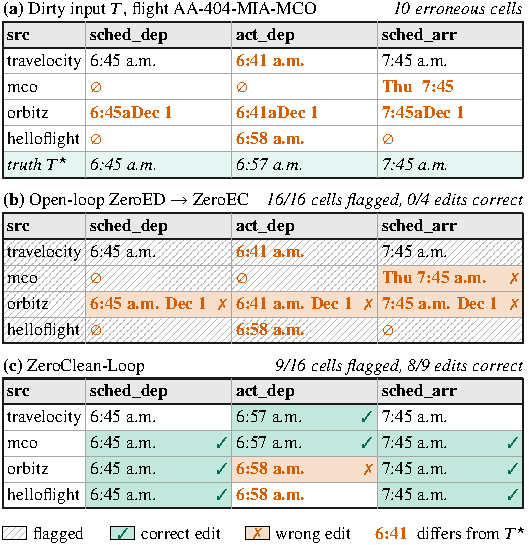
\includegraphics[width=\columnwidth]{figures/fig_example.pdf}
\caption{Running example from the Flights benchmark, three time attributes in four of the 27 source reports of flight AA-404-MIA-MCO: (a) dirty input $T$ and the evaluator-only reference $T^{\star}$; (b) output of the open-loop cascade of ZeroED and ZeroEC; (c) output of ZeroClean-Loop. Hatching marks a flagged cell, green with a check mark marks an edit that equals $T^{\star}$, vermilion with a cross marks an edit that differs from $T^{\star}$, bold vermilion text marks a value that differs from $T^{\star}$, and $\varnothing$ marks an empty cell.}
\label{fig:example}
\end{figure}

\begin{figure*}[t]
\centering
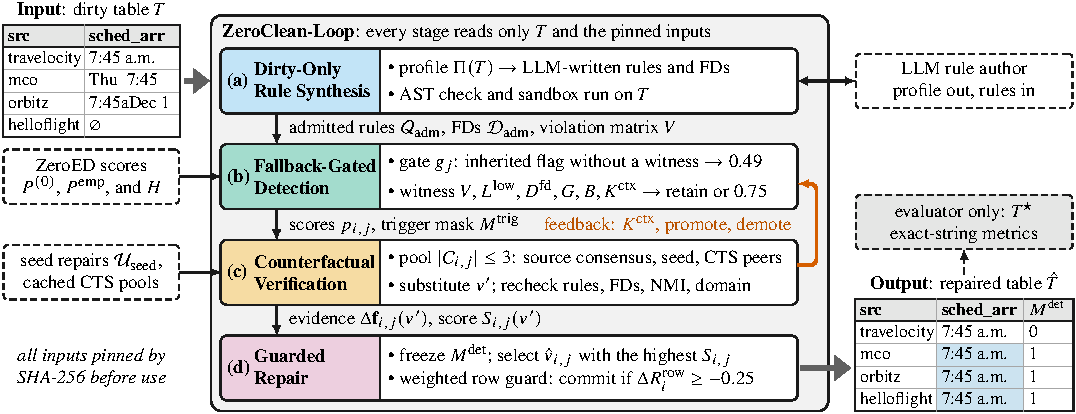
\includegraphics[width=\textwidth]{figures/fig_overview.pdf}
\caption{Data flow of ZeroClean-Loop through four coupled stages: (a) dirty-only rule synthesis, which turns a stratified profile of $T$ into sandbox-validated rules and FDs; (b) fallback-gated detection, which gates inherited scores with dirty-only witnesses; (c) counterfactual verification, which substitutes every candidate into a copy of its tuple; (d) guarded repair, which freezes the mask and commits rows that pass the weighted guard. The left table shows one attribute of the running example in $T$, and the right table shows the same cells in the repaired table $\hat{T}$ with the frozen mask $M^{\mathrm{det}}$; blue cells are committed edits. Black arrows carry the artifacts between stages, the vermilion arrow carries repair-side evidence back to detection, dashed boxes are pinned inputs and the LLM rule author, and the grey box is the evaluator, which is the only component that reads $T^{\star}$.}
\label{fig:overview}
\end{figure*}

\subsection{Failure of Open-Loop Zero-Shot Pipelines}
\label{subsec:intro_gap}

Recent foundation-model approaches remove manual labeling by splitting zero-shot cleaning into two standalone phases. ZeroED~\cite{ni2025zeroed} asks a Large Language Model (LLM) to write executable verification functions and trains per-column classifiers for Error Detection (ED). ZeroEC~\cite{chen2025zeroec} applies Contextual Tuple Search (CTS) to retrieve peer tuples and prompts an LLM for Error Correction (EC) on the flagged cells. Fig.~\ref{fig:example} shows what the sequential cascade of the two systems produces on four reports of one flight. The dirty input in Fig.~\ref{fig:example}(a) contains 10 erroneous cells among the 12 time values. In Fig.~\ref{fig:example}(b), the detector flags all 16 displayed cells, including the source names, and the repairer edits four cells; every edit rewrites the surface form of the dirty value (for example \texttt{Thu 7:45} becomes \texttt{Thu 7:45 a.m.}) and none equals the reference value. This behavior follows from three architectural defects:

\begin{enumerate}[leftmargin=*, itemsep=0pt, topsep=1pt]
\item \textbf{Empty-Predicate Classifier Degeneracy.} ZeroED samples $5~\%$ of the dirty tuples as cluster representatives, asks an LLM to label errors, and synthesizes error-conditioned Python predicates. When the sampled representatives of a column contain no labeled error, the predicate set is empty. The clean-label filter divides the number of satisfied criteria by the criterion count plus $10^{-6}$, obtains zero, and discards every propagated clean training example. The per-column Multi-Layer Perceptron (MLP) is then trained on synthetic error examples only and predicts every cell of the column as dirty. On the six benchmark tables, source ZeroED flags all 14,256 cells of Flights, 17,208 of the 21,690 cells of Beers, and 110,873 of the 125,630 cells of Movies, and its macro detection score is \SourceMacroED{}.
\item \textbf{Unguarded Candidate Substitution.} An over-inclusive mask forces the repairer to propose edits for thousands of clean cells, and no consistency check stands between a proposed value and the output table. On Flights, the sequential cascade edits 295 cells and four edits equal the reference value, which yields a repair score of 0.0015.
\item \textbf{No Feedback Between Repair and Detection.} In a one-way pipeline, the detector never observes whether a flagged cell admits a consistent repair, and the repairer has no channel to report that an unflagged cell contradicts the value on which the other sources of the same entity agree.
\end{enumerate}

\subsection{Closed-Loop Counterfactual Cleaning}
\label{subsec:intro_novelty}

This work formulates autonomous tabular cleaning as a \emph{closed-loop counterfactual verification problem} over the immutable dirty table $T$. Fig.~\ref{fig:overview} shows the data flow. Stage (a) synthesizes executable rules and Functional Dependencies (FDs) from a bounded dirty profile and validates them in a sandbox. Stage (b) audits the inherited classifier scores per column: when a column exhibits the empty-predicate degeneracy, an inherited flag survives only if an independent dirty-only witness corroborates it. Stage (c) treats each candidate value as a concrete intervention on its tuple: the system substitutes the value, re-executes the rules, and recomputes FD support, vicinity likelihood, and domain support, which yields a four-dimensional change vector. Evidence produced for repair returns to stage (b) before the mask is frozen. Stage (d) selects the best eligible candidate per flagged cell and commits a row only when the jointly edited tuple passes a weighted rule guard. In Fig.~\ref{fig:example}(c), this procedure flags 9 of the 16 displayed cells, all of them erroneous, and commits 9 edits of which 8 equal the reference value; one erroneous cell of the fourth report remains undetected, and Section~\ref{subsec:exp_diagnostics} quantifies this failure mode.

\subsection{Summary of Contributions}
\label{subsec:intro_contributions}

\begin{itemize}[leftmargin=*, itemsep=0pt, topsep=1pt]
\item \textbf{Closed-Loop Formulation (Section~\ref{sec:preliminaries}).} We formalize zero-shot tabular cleaning under a dirty-only information boundary and define the coupling between mask revision and counterfactual candidate verification.
\item \textbf{Fallback-Gated Intrinsic Detection (Section~\ref{sec:detection}).} We diagnose the empty-predicate failure of LLM-guided detectors and design a column gate, a leave-one-out support profile, a single-determinant FD discovery procedure with a marginal purity gain bound, and two structural promoters.
\item \textbf{Consensus and Counterfactual Repair (Section~\ref{sec:repair}).} We develop a key-grouped source consensus estimator for multi-source tables, a four-feature counterfactual scorer, and an inverse-violation weighted whole-row guard.
\item \textbf{Parallel and Progressive Evaluation (Section~\ref{sec:experiments}).} We evaluate ZeroClean-Loop on six datasets (16,790 tuples, 247,084 cells, and 23,277 erroneous cells) against source, adapted, sequential, and seeded baselines and across six frozen study cohorts. ZeroClean-Loop v6 improves the macro detection score by \VsixEDGain{} (percentage points) and the macro repair score by \VsixRepairGain{}. We report with equal weight where the method loses: v6 gives up 31.23~pp of detection score on Rayyan relative to v4, $79.8~\%$ of its Beers edits are wrong under exact-string evaluation, and the two counterfactual feedback rules change no cell on the six benchmarks.
\end{itemize}

\section{Preliminaries and Protocol Boundary}
\label{sec:preliminaries}

\subsection{Relational Error Model and Cleaning Objectives}
\label{subsec:prelim_model}

Let $T = (R, C)$ denote an observed dirty relational table with $n = |R|$ tuples $R = (r_1, \dots, r_n)$ over $m = |C|$ attribute columns $C = (c_1, \dots, c_m)$. Each cell at row $i$ and column $j$ stores a dirty string $x_{i,j} \in \Sigma^{\star}$, where $\Sigma^{\star}$ denotes the set of finite Unicode strings including the empty string $\varepsilon$. A reference table $T^{\star} = (R^{\star}, C)$ of identical dimension exists only in the external evaluation environment, with clean string $x_{i,j}^{\star} \in \Sigma^{\star}$ at each coordinate. The true error indicator matrix $E^{\star} \in \{0,1\}^{n \times m}$ and the error set $\mathcal{E}^{\star}$ are defined as
\begin{equation}
\label{eq:truth_def}
\left\{
\begin{aligned}
E_{i,j}^{\star} &= \mathbb{I}\!\left[x_{i,j} \neq x_{i,j}^{\star}\right], \\
\mathcal{E}^{\star} &= \left\{(i,j) \;\middle|\; E_{i,j}^{\star} = 1\right\},
\end{aligned}
\right.
\end{equation}
where $E_{i,j}^{\star} \in \{0,1\}$ is the corruption label of cell $(i,j)$, $\mathbb{I}[\cdot]$ is the indicator function that returns $1$ when its predicate holds and $0$ otherwise, $x_{i,j}$ is the observed dirty string, $x_{i,j}^{\star}$ is the clean reference string, and $\mathcal{E}^{\star}$ is the set of all corrupted cell coordinates.

A cleaning system outputs a triple $(P, M^{\mathrm{det}}, \mathcal{U})$, where $P = [p_{i,j}] \in [0,1]^{n \times m}$ is a matrix of detection scores, $M^{\mathrm{det}} \in \{0,1\}^{n \times m}$ is the frozen binary detection mask, and $\mathcal{U} : \mathcal{S}_{\mathrm{rep}} \to \Sigma^{\star}$ is a sparse repair mapping over a subset $\mathcal{S}_{\mathrm{rep}}$ of the flagged coordinates. The detection decision and the emitted cell value $\hat{x}_{i,j}$ are governed by
\begin{equation}
\label{eq:mask_repair_def}
\left\{
\begin{aligned}
M_{i,j}^{\mathrm{det}} &= \mathbb{I}\!\left[p_{i,j} > \tau_{\mathrm{det}}\right], \\
\hat{x}_{i,j} &=
\begin{cases}
\hat{v}_{i,j}, & \text{if } (i,j) \in \mathcal{S}_{\mathrm{rep}}, \\
x_{i,j}, & \text{otherwise},
\end{cases}
\end{aligned}
\right.
\end{equation}
where $p_{i,j} \in [0,1]$ is the detection score of cell $(i,j)$, $\tau_{\mathrm{det}} = 0.50$ is the strict decision threshold, $\hat{x}_{i,j}$ is the emitted string, $\hat{v}_{i,j} = \mathcal{U}(i,j) \neq x_{i,j}$ is the committed replacement string, and $\mathcal{S}_{\mathrm{rep}} \subseteq \{(i,j) \mid M_{i,j}^{\mathrm{det}} = 1\}$ is the set of repaired coordinates.

The evaluator compares $(M^{\mathrm{det}}, \mathcal{U})$ with $T^{\star}$ by exact string equality without whitespace stripping, case folding, or numerical coercion. For ED, the counts of True Positives (TP), False Positives (FP), and False Negatives (FN) and the resulting precision, recall, and $F_1$ score are
\begin{equation}
\label{eq:ed_metrics}
\left\{
\begin{aligned}
\mathrm{TP}^{\mathrm{ED}} &= \sum_{i=1}^{n}\sum_{j=1}^{m} \mathbb{I}\!\left[M_{i,j}^{\mathrm{det}} = 1 \land E_{i,j}^{\star} = 1\right], \\
\mathrm{FP}^{\mathrm{ED}} &= N_{\mathrm{pos}} - \mathrm{TP}^{\mathrm{ED}}, \quad
\mathrm{FN}^{\mathrm{ED}} = \left|\mathcal{E}^{\star}\right| - \mathrm{TP}^{\mathrm{ED}}, \\
P^{\mathrm{ED}} &= \frac{\mathrm{TP}^{\mathrm{ED}}}{N_{\mathrm{pos}}}, \quad
R^{\mathrm{ED}} = \frac{\mathrm{TP}^{\mathrm{ED}}}{\left|\mathcal{E}^{\star}\right|}, \\
F_1^{\mathrm{ED}} &= \frac{2 P^{\mathrm{ED}} R^{\mathrm{ED}}}{P^{\mathrm{ED}} + R^{\mathrm{ED}}},
\end{aligned}
\right.
\end{equation}
where $N_{\mathrm{pos}} = \sum_{i,j} M_{i,j}^{\mathrm{det}}$ is the number of flagged cells, $\mathrm{TP}^{\mathrm{ED}}$, $\mathrm{FP}^{\mathrm{ED}}$, and $\mathrm{FN}^{\mathrm{ED}}$ are the cell-level detection counts, and $P^{\mathrm{ED}}, R^{\mathrm{ED}}, F_1^{\mathrm{ED}} \in [0,1]$ are detection precision, recall, and $F_1$ score.

For EC, every edited cell is compared with $x_{i,j}^{\star}$, and every erroneous cell that stays unedited or receives a wrong replacement counts as a false negative. A wrong edit on an erroneous cell is therefore both a repair false positive and a repair false negative:
\begin{equation}
\label{eq:ec_metrics}
\left\{
\begin{aligned}
\mathrm{TP}^{\mathrm{EC}} &= \sum_{(i,j) \in \mathcal{S}_{\mathrm{rep}}} \mathbb{I}\!\left[E_{i,j}^{\star} = 1 \land \hat{v}_{i,j} = x_{i,j}^{\star}\right], \\
P^{\mathrm{EC}} &= \frac{\mathrm{TP}^{\mathrm{EC}}}{\left|\mathcal{S}_{\mathrm{rep}}\right|}, \quad
R^{\mathrm{EC}} = \frac{\mathrm{TP}^{\mathrm{EC}}}{\left|\mathcal{E}^{\star}\right|}, \\
F_1^{\mathrm{EC}} &= \frac{2 P^{\mathrm{EC}} R^{\mathrm{EC}}}{P^{\mathrm{EC}} + R^{\mathrm{EC}}},
\end{aligned}
\right.
\end{equation}
where $\mathrm{TP}^{\mathrm{EC}}$ is the number of edits that equal the reference string, $|\mathcal{S}_{\mathrm{rep}}|$ is the number of edits, and $P^{\mathrm{EC}}, R^{\mathrm{EC}}, F_1^{\mathrm{EC}} \in [0,1]$ are repair precision, recall, and $F_1$ score. Over a benchmark cohort $\mathcal{B}$, the unweighted macro averages are
\begin{equation}
\label{eq:macro_f1}
\left\{
\begin{aligned}
\bar{F}_1^{\mathrm{ED}} &= \frac{1}{\left|\mathcal{B}\right|} \sum_{b \in \mathcal{B}} F_{1,b}^{\mathrm{ED}}, \\
\bar{F}_1^{\mathrm{EC}} &= \frac{1}{\left|\mathcal{B}\right|} \sum_{b \in \mathcal{B}} F_{1,b}^{\mathrm{EC}},
\end{aligned}
\right.
\end{equation}
where $\mathcal{B}$ is the cohort of $|\mathcal{B}| = 6$ datasets, $F_{1,b}^{\mathrm{ED}}$ and $F_{1,b}^{\mathrm{EC}}$ are the detection and repair scores on dataset $b$, and $\bar{F}_1^{\mathrm{ED}}, \bar{F}_1^{\mathrm{EC}} \in [0,1]$ are the macro averages.

\subsection{Dirty-Only Information Boundary and Sandboxed Rules}
\label{subsec:prelim_boundary}

ZeroClean-Loop separates inference from evaluation (frame and grey box of Fig.~\ref{fig:overview}). For each dataset, the inference runner receives nine immutable inputs that are pinned by the Secure Hash Algorithm 256-bit (SHA-256) digest, which amounts to 54 files over the cohort: (1) the dirty table $T$ as a Comma-Separated Values (CSV) file; (2) the source ZeroED scores $P^{(0)} = [p_{i,j}^{(0)}]$ with the classifier metadata $H$; (3) the carry scores $P^{\mathrm{emp}} = [p_{i,j}^{\mathrm{emp}}]$ of the empty-state verification arm (Section~\ref{subsec:exp_setup}); (4) the sequential seed repairs $\mathcal{U}_{\mathrm{seed}}$; (5) the cached CTS candidate pools; (6) a bounded dirty profile $\Pi(T)$ with frequent, rare, and diverse tuple strata; (7) the raw JavaScript Object Notation (JSON) response of the LLM; (8) the fresh rule artifact; and (9) the previously cached rule artifact. No inference module reads a clean reference file, an oracle mask, an external catalog, or an evaluation failure log.

From $\Pi(T)$, the LLM writes candidate Python rules $q_k : \Sigma^{\star m} \to \{-1, 0, 1\}$, where $1$ signals a violation, $0$ satisfaction, and $-1$ a runtime exception, together with candidate FD declarations. Every rule passes an Abstract Syntax Tree (AST) check that forbids imports, dunder attributes, and input or output calls, and then executes over all dirty tuples in batches of 1,000~tuples inside a resource-bounded subprocess confined by the Linux Secure Computing Mode (seccomp). Let $z_{i,k} = q_k(r_i)$. The runtime error rate $\epsilon_k$, the violation rate $\nu_k$, the admitted rule set $\mathcal{Q}_{\mathrm{adm}}$, and the rule violation matrix $V$ are
\begin{equation}
\label{eq:rule_admission}
\left\{
\begin{aligned}
\epsilon_k &= \frac{1}{n}\sum_{i=1}^{n} \mathbb{I}\!\left[z_{i,k} = -1\right], \quad
\nu_k = \frac{\sum_{i} \mathbb{I}\!\left[z_{i,k} = 1\right]}{\sum_{i} \mathbb{I}\!\left[z_{i,k} \ge 0\right]}, \\
\mathcal{Q}_{\mathrm{adm}} &= \left\{q_k \;\middle|\; \epsilon_k < \tau_{\mathrm{err}} \right\}, \\
V_{i,j} &= \mathbb{I}\!\left[\exists q_k \in \mathcal{Q}_{\mathrm{adm}} : c_j \in \mathcal{T}(q_k) \land \nu_k < 1 \land z_{i,k} = 1\right],
\end{aligned}
\right.
\end{equation}
where $z_{i,k} \in \{-1,0,1\}$ is the sandboxed output of rule $q_k$ on tuple $r_i$, $\epsilon_k \in [0,1]$ is the fraction of tuples that raise an exception, $\tau_{\mathrm{err}} = 0.05$ is the admission ceiling of $5~\%$, $\nu_k \in [0,1]$ is the violation fraction among the tuples that execute, $\mathcal{T}(q_k) \subseteq C$ is the target column set of $q_k$, and $V_{i,j} \in \{0,1\}$ indicates that cell $(i,j)$ violates an admitted rule that targets $c_j$. A rule with $\nu_k = 1$ fires on every tuple and is excluded from $V$; a rule with $\nu_k = 0$ never fires on $T$ and stays in $\mathcal{Q}_{\mathrm{adm}}$ as a guard against invalid candidate repairs.

\section{Fallback-Gated and Intrinsic Error Detection}
\label{sec:detection}

\subsection{Fallback Gating of Inherited Classifier Scores}
\label{subsec:det_gating}

The detector starts from the inherited scores and first decides, per column, whether they are trustworthy. From the metadata $H_j$ of column $c_j$ it reads the fallback indicator $\mathrm{fb}_j \in \{0,1\}$, which equals $1$ when the clean predicate count after filtering is zero or the single-class MLP fallback is recorded, and it computes the source positive fraction $\gamma_j$:
\begin{equation}
\label{eq:gate_trigger}
\left\{
\begin{aligned}
\gamma_j &= \frac{1}{n}\sum_{i=1}^{n} \mathbb{I}\!\left[p_{i,j}^{(0)} > \tau_{\mathrm{det}}\right], \\
g_j &= \mathbb{I}\!\left[\mathrm{fb}_j = 1 \;\lor\; \gamma_j > \tau_{\mathrm{src}}\right],
\end{aligned}
\right.
\end{equation}
where $\gamma_j \in [0,1]$ is the fraction of tuples that the source detector flags in column $c_j$, $\mathrm{fb}_j$ is the empty-predicate fallback flag, $\tau_{\mathrm{src}} = 0.40$ is the gating threshold, and $g_j \in \{0,1\}$ indicates that column $c_j$ is gated.

In a gated column, an inherited positive ($p_{i,j}^{\mathrm{emp}} > \tau_{\mathrm{det}}$) is retained only if at least one independent dirty-only witness corroborates it: a rule violation ($V_{i,j} = 1$), a leave-one-out rarity signal ($L_{i,j}^{\mathrm{low}} = 1$), or a contradiction with the source consensus of the same entity ($K_{i,j}^{\mathrm{ctx}} = 1$, Section~\ref{subsec:rep_consensus}). An unsupported inherited positive is demoted to $p_{\mathrm{dem}} = 0.49$, immediately below $\tau_{\mathrm{det}}$, which removes it from the mask and keeps it inside the uncertainty interval that triggers candidate generation.

\begin{figure*}[t]
\centering
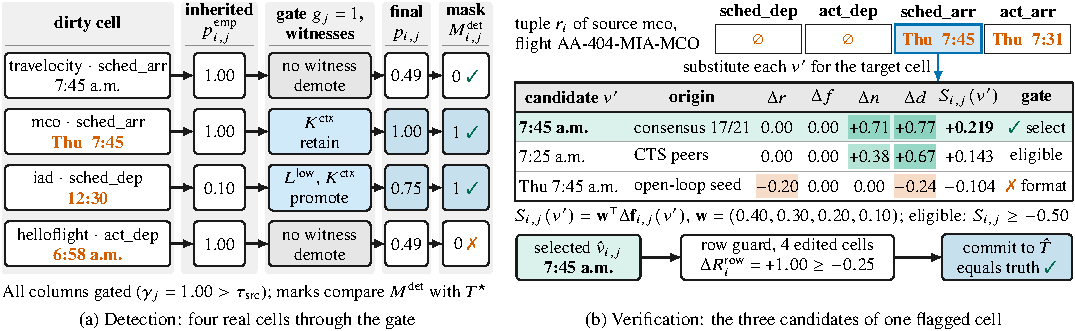
\includegraphics[width=\textwidth]{figures/fig_trace.pdf}
\caption{Execution traces of real Flights cells, read from the frozen audit log: (a) detection of four cells, from the inherited score $p_{i,j}^{\mathrm{emp}}$ through the column gate $g_j$ and the dirty-only witnesses to the final score $p_{i,j}$ and the mask $M_{i,j}^{\mathrm{det}}$; (b) counterfactual verification of the three candidates $v'$ of one flagged cell, with the four feature changes $\Delta r$, $\Delta f$, $\Delta n$, and $\Delta d$, the score $S_{i,j}(v')$, and the weighted whole-row guard. Blue marks retained or promoted flags, grey marks demoted flags, green marks positive and orange marks negative feature changes, and check marks and crosses compare the outcome with $T^{\star}$.}
\label{fig:trace}
\end{figure*}

Fig.~\ref{fig:trace}(a) follows four cells of the running example through the gate. All six Flights columns are gated because source ZeroED flags every cell ($\gamma_j = 1.00$). The correct arrival time \texttt{7:45 a.m.} has no witness and is demoted from 1.00 to 0.49. The malformed value \texttt{Thu 7:45} contradicts the source consensus and stays flagged. The value \texttt{12:30}, which carries an inherited score of 0.10, has low leave-one-out support and contradicts the consensus, so it is promoted to 0.75. The erroneous departure time \texttt{6:58 a.m.} is well formed, violates no rule, and has no actionable consensus alternative; it is demoted and becomes a false negative.

\subsection{Leave-One-Out Support and Single-Determinant FDs}
\label{subsec:det_intrinsic}

Every column statistic excludes the query cell itself; otherwise a singleton error contributes to its own support. Let $\sigma(x)$ denote the coarse format signature of a string, which maps alphabetic runs to \texttt{A}, digit runs to \texttt{9}, and signed decimal or scientific literals to \texttt{numeric}. Let $n_j^{+}$ be the number of non-empty cells of column $c_j$ and $n_{i,j}^{\mathrm{peer}} = n_j^{+} - \mathbb{I}[x_{i,j} \neq \varepsilon]$ the non-empty peer count. The value peer count, the format peer count, and the low-support indicator are
\begin{equation}
\label{eq:loo_support}
\left\{
\begin{aligned}
c_{i,j}^{\mathrm{val}} &= \sum_{r \neq i} \mathbb{I}\!\left[x_{r,j} = x_{i,j} \land x_{i,j} \neq \varepsilon\right], \\
c_{i,j}^{\mathrm{fmt}} &= \sum_{r \neq i} \mathbb{I}\!\left[\sigma(x_{r,j}) = \sigma(x_{i,j}) \land x_{i,j} \neq \varepsilon\right], \\
L_{i,j}^{\mathrm{low}} &= \mathbb{I}\!\left[\bigvee_{u \in \{\mathrm{fmt}, \mathrm{val}\}} \left(\phi_j^{u} = 1 \land c_{i,j}^{u} \le \kappa_{\mathrm{rare}} \land \frac{c_{i,j}^{u}}{n_{i,j}^{\mathrm{peer}}} \le \rho_{\mathrm{rare}}\right)\right],
\end{aligned}
\right.
\end{equation}
where $c_{i,j}^{\mathrm{val}}$ and $c_{i,j}^{\mathrm{fmt}}$ are the leave-one-out peer counts of the exact value and of the format signature, $n_{i,j}^{\mathrm{peer}}$ is the non-empty peer count, $\kappa_{\mathrm{rare}} = 1$ is the maximum rare peer count, $\rho_{\mathrm{rare}} = 0.02$ is the maximum rare peer fraction, and $\phi_j^{\mathrm{fmt}}, \phi_j^{\mathrm{val}} \in \{0,1\}$ are comparability gates of column $c_j$. The format gate $\phi_j^{\mathrm{fmt}} = 1$ requires at least 8 peers, a structured peer fraction of at least 0.90, and a dominant signature that covers at least 0.90 of the peers. The value gate $\phi_j^{\mathrm{val}} = 1$ requires at least 30 peers, a distinct value fraction of at most 0.20, and a mass of at least 0.90 on values that occur at least 3 times.

ZeroClean-Loop also discovers single-determinant FDs $c_k \to c_j$ from repeated dirty groups. Let $\mathcal{G}_k$ denote the groups of tuples that share a non-empty determinant value in $c_k$ and hold at least 4 non-empty observations of $c_j$. For each group $g$, let $c_{g,j}^{\max}$ be the frequency of the modal value of $c_j$. The relational purity and the marginal purity are
\begin{equation}
\label{eq:fd_purity}
\left\{
\begin{aligned}
\pi_{k \to j} &= \frac{\sum_{g \in \mathcal{G}_k} c_{g,j}^{\max}}{\sum_{g \in \mathcal{G}_k} |g|}, \\
\pi_{k \to j}^{\mathrm{marg}} &= \frac{\max_{v \in \Sigma^{\star}} \sum_{g \in \mathcal{G}_k} \sum_{r \in g} \mathbb{I}[x_{r,j} = v]}{\sum_{g \in \mathcal{G}_k} |g|},
\end{aligned}
\right.
\end{equation}
where $\mathcal{G}_k$ is the set of repeated determinant groups of column $c_k$, $c_{g,j}^{\max}$ is the modal frequency of $c_j$ within group $g$, $\pi_{k \to j} \in [0,1]$ is the conditional purity of $c_k \to c_j$, and $\pi_{k \to j}^{\mathrm{marg}} \in [0,1]$ is the purity of the single most frequent value over the covered tuples. An FD is admitted when $|\mathcal{G}_k| \ge 2$, the groups cover at least 0.15 of the observations, $\pi_{k \to j} \ge 0.97$, the groups exhibit at least two distinct modes, and $\pi_{k \to j} - \pi_{k \to j}^{\mathrm{marg}} \ge 0.10$. The gain bound prevents a nearly constant column from turning every attribute into a determinant. On Hospital, the FD from the provider number to the hospital name has 42 groups over 967 observations with purity 0.9752 against a marginal purity of 0.0279. A cell receives the FD witness $D_{i,j}^{\mathrm{fd}} = 1$ when all admitted determinants that cover tuple $i$ agree on one peer mode, with at least $95~\%$ agreement within the group over at least 3 peers, and that mode differs from $x_{i,j}$.

\subsection{Generic and Fallback Structural Promotion}
\label{subsec:det_structural}

Two structural promoters capture corruptions that escape the LLM rules (stage (b) of Fig.~\ref{fig:overview}):
\begin{enumerate}[leftmargin=*, itemsep=0pt, topsep=1pt]
\item \textbf{Complete-Column Format Outliers ($G_{i,j}$).} In a column with coverage $\eta_j = n_j^{+} / n \ge 0.98$, at least 30 non-empty cells, and a dominant format share of at least 0.90, every cell that is empty or deviates from the dominant signature receives $G_{i,j} = 1$.
\item \textbf{Fallback-Column Grammar ($B_{i,j}$).} In a fallback column ($\mathrm{fb}_j = 1$) with $\eta_j \ge 0.45$, the detector fits a family of grammars (hyphenated serial numbers, page ranges, numbers, and calendar dates) to the non-empty values. When at least 8 values exist and the best grammar covers at least 0.80 of them, a non-empty cell that violates the grammar receives $B_{i,j} = 1$. When $\eta_j \ge 0.80$ and the column is not an open-vocabulary attribute, an empty cell also receives $B_{i,j} = 1$.
\end{enumerate}
The open-vocabulary test combines a distinct value fraction of at least 0.35 with a list of column-name tokens such as \texttt{title} and \texttt{description}; this list is the one place where v6 consults column names, and Section~\ref{subsec:exp_diagnostics} returns to it. Together with checks for control characters, inferred type contradictions (at least $95~\%$ valid peers), and case or spacing variants of a compact domain, every cell with an active witness is promoted to $\max(p_{i,j}, p_{\mathrm{prom}})$ with $p_{\mathrm{prom}} = 0.75$.

\section{Counterfactual Verification and Consensus Repair}
\label{sec:repair}

\subsection{Key-Grouped Source Consensus and Candidate Pool}
\label{subsec:rep_consensus}

In a multi-source table such as Flights, several sources report the same entity, and whole-tuple CTS retrieval returns tuples of other entities. ZeroClean-Loop discovers an entity key $K_{\mathrm{ent}} \subset C$ with $|K_{\mathrm{ent}}| \le 2$ and a source column $c_{\mathrm{src}}$ from tuple multiplicities: a configuration is valid when at least two entities repeat, at least 0.50 of the entities have several sources, and at least 0.80 of the entity and source pairs hold one tuple. For each source $s$ with tuple set $R_s$, the module combines three dirty-only signals, namely format validity $f_s^{\mathrm{fmt}}$, chronological consistency $f_s^{\mathrm{chr}}$ (departure precedes arrival), and peer agreement $f_s^{\mathrm{peer}}$. The source weight and the weighted consensus support of a candidate $v'$ are
\begin{equation}
\label{eq:source_consensus}
\left\{
\begin{aligned}
q_s^{\mathrm{raw}} &= \beta_{\mathrm{peer}} f_s^{\mathrm{peer}} + \beta_{\mathrm{fmt}} f_s^{\mathrm{fmt}} + \beta_{\mathrm{chr}} f_s^{\mathrm{chr}}, \\
w_s &= \max\!\left(w_{\min},\; \frac{\lambda_0 \bar{q} + |R_s| q_s^{\mathrm{raw}}}{\lambda_0 + |R_s|}\right), \\
A_{i,j}(v') &= \frac{\sum_{s \in \mathcal{S}_{i}} w_s \,\mathbb{I}\!\left[v_{s,j} = v'\right]}{\sum_{s \in \mathcal{S}_{i}} w_s},
\end{aligned}
\right.
\end{equation}
where $q_s^{\mathrm{raw}} \in [0,1]$ is the raw quality of source $s$, $\beta_{\mathrm{peer}} = 0.50$, $\beta_{\mathrm{fmt}} = 0.35$, and $\beta_{\mathrm{chr}} = 0.15$ are the signal weights, $\bar{q}$ is the mean quality over all sources, $\lambda_0 = 3.0$ is the prior strength, $w_{\min} = 0.20$ is the reliability floor, $w_s \in [w_{\min}, 1]$ is the shrunk reliability weight, $\mathcal{S}_{i}$ is the set of peer sources that report the entity of tuple $i$ without the source of tuple $i$ itself, $v_{s,j}$ is the value that source $s$ reports for column $c_j$, and $A_{i,j}(v') \in [0,1]$ is the weighted agreement. A candidate is \emph{actionable} when it is the unique winner under both unweighted source counts and weighted votes, at least 2 peer sources support it, $A_{i,j}(v') \ge 2/3$, the weighted margin over the runner-up is at least 0.20, and the edited tuple passes the format and chronology checks. The consensus contradiction witness of Section~\ref{subsec:det_gating} is $K_{i,j}^{\mathrm{ctx}} = 1$ when an actionable candidate $v' \neq x_{i,j}$ exists.

Candidate pools are built for every cell of the trigger mask
\begin{equation}
\label{eq:trigger_mask}
M_{i,j}^{\mathrm{trig}} = \mathbb{I}\!\left[p_{i,j} > \tau_{\mathrm{det}} \;\lor\; \tau_{\mathrm{low}} \le p_{i,j} \le \tau_{\mathrm{high}}\right],
\end{equation}
where $M_{i,j}^{\mathrm{trig}} \in \{0,1\}$ is the trigger indicator, $p_{i,j}$ is the detection score after gating and promotion, and $[\tau_{\mathrm{low}}, \tau_{\mathrm{high}}] = [0.25, 0.85]$ is the uncertainty interval. The pool $\mathcal{C}_{i,j}$ of a triggered cell holds at most $K_{\max} = 3$ distinct strings $v' \neq x_{i,j}$ in a fixed priority order: actionable consensus values, seed proposals from $\mathcal{U}_{\mathrm{seed}}$, and CTS peer values. The system never synthesizes a string outside the observed dirty values and the seed proposals.

\subsection{Four-Dimensional Counterfactual Features}
\label{subsec:rep_counterfactual}

For each candidate $v' \in \mathcal{C}_{i,j}$, ZeroClean-Loop builds the counterfactual tuple $r_i^{(j \leftarrow v')}$, which replaces $x_{i,j}$ by $v'$ and keeps every other attribute at its dirty value (stage (c) of Fig.~\ref{fig:overview}). Let $\mathcal{Q}_j(i, v')$ denote the admitted rules that target $c_j$ and execute without exception on both $r_i$ and $r_i^{(j \leftarrow v')}$. The change vector $\Delta\mathbf{f}_{i,j}(v') = (\Delta r, \Delta f, \Delta n, \Delta d)^{\top}$ and the consistency score are
\begin{equation}
\label{eq:counterfactual_vector}
\left\{
\begin{aligned}
\Delta r_{i,j}(v') &= \frac{\sum_{q_k \in \mathcal{Q}_j(i, v')} \!\left(q_k(r_i) - q_k\!\left(r_i^{(j \leftarrow v')}\right)\right)}{\max\!\left(1, |\mathcal{Q}_j(i, v')|\right)}, \\
\Delta f_{i,j}(v') &= \Psi_{\mathrm{fd}}\!\left(v', r_i^{(j \leftarrow v')}\right) - \Psi_{\mathrm{fd}}\!\left(x_{i,j}, r_i\right), \\
\Delta n_{i,j}(v') &= \tanh\!\left(\frac{\Psi_{\mathrm{vic}}\!\left(v', r_i^{(j \leftarrow v')}\right) - \Psi_{\mathrm{vic}}\!\left(x_{i,j}, r_i\right)}{\kappa_{\mathrm{scale}}}\right), \\
\Delta d_{i,j}(v') &= \tanh\!\left(\frac{\Psi_{\mathrm{dom}}(v') - \Psi_{\mathrm{dom}}(x_{i,j})}{\kappa_{\mathrm{scale}}}\right), \\
S_{i,j}(v') &= \mathbf{w}^{\top} \Delta\mathbf{f}_{i,j}(v'),
\end{aligned}
\right.
\end{equation}
where $\Delta r_{i,j}(v') \in [-1,1]$ is the normalized reduction of rule violations, $\Psi_{\mathrm{fd}}(v, r) \in [0,1]$ is the leave-one-out conditional support of value $v$ in column $c_j$ under the declared FDs given tuple $r$, $\Delta f_{i,j}(v')$ is the gain in FD support, $\Psi_{\mathrm{vic}}(v, r)$ is the co-occurrence log-likelihood of $v$ with the context attributes of $r$ weighted by Normalized Mutual Information (NMI), $\Delta n_{i,j}(v')$ is the vicinity gain, $\Psi_{\mathrm{dom}}(v)$ is the leave-one-out log-frequency and pattern support of $v$ in column $c_j$, $\Delta d_{i,j}(v')$ is the domain gain, $\kappa_{\mathrm{scale}} = 4.0$ is the scaling divisor of the hyperbolic tangent, $\mathbf{w} = (0.40, 0.30, 0.20, 0.10)^{\top}$ is the fixed weight vector, and $S_{i,j}(v') \in [-1,1]$ is the weighted consistency score.

Fig.~\ref{fig:trace}(b) shows the three candidates of the cell \texttt{Thu 7:45}. The value \texttt{7:45 a.m.} is the actionable consensus value, reported by 17 of the 21 peer sources with $A_{i,j} = 0.86$, and CTS returns it as well; it raises vicinity and domain support ($\Delta n = +0.71$, $\Delta d = +0.77$) and scores $S_{i,j} = +0.219$. The CTS peer value \texttt{7:25 a.m.} scores $+0.143$. The seed edit \texttt{Thu 7:45 a.m.} of the sequential baseline lowers rule satisfaction and domain support ($\Delta r = -0.20$, $\Delta d = -0.24$), scores $-0.104$, and fails the format check.

Repair-side evidence reaches the detector through three channels before the mask is frozen (vermilion arrow in Fig.~\ref{fig:overview}):
\begin{enumerate}[leftmargin=*, itemsep=0pt, topsep=1pt]
\item \textbf{Consensus Contradiction.} The witness $K_{i,j}^{\mathrm{ctx}}$ corroborates an inherited flag or promotes an unflagged cell (Section~\ref{subsec:det_gating}).
\item \textbf{Counterfactual Promotion.} Let $v^{\star}$ be the viable candidate with the largest feature sum. An unflagged triggered cell is promoted to $\max(p_{i,j}, 0.75)$ when $v^{\star}$ reduces rule violations ($\Delta r > 0$) and is actionable or has $A_{i,j}(v^{\star}) \ge 0.66$, or when $v^{\star}$ raises FD support ($\Delta f > 0$) and is format-valid.
\item \textbf{Counterfactual Demotion.} A flagged cell is demoted to $\min(p_{i,j}, 0.49)$ when $v^{\star}$ is format-invalid with $\Delta d < 0$ and every viable candidate lowers all four features.
\end{enumerate}
On the six benchmark tables, the first channel carries the entire measured feedback; the second and third rules are part of the frozen system and change no cell (Section~\ref{subsec:exp_diagnostics}).

\subsection{Weighted Whole-Row Consistency Guard}
\label{subsec:rep_rowguard}

After the mask is frozen and set read-only, the selector reviews the candidates of every flagged cell. A candidate is eligible when it raises no sandbox exception, is format-valid, does not contradict a unanimous leave-one-out FD value, and satisfies $S_{i,j}(v') \ge \tau_{\mathrm{loss}} = -0.50$. It also needs positive evidence: a seed origin, actionable consensus, a strict witness (FD consensus, CTS peer agreement, or $\Delta r > 0$), or $S_{i,j}(v') > 0$. The selector picks the eligible candidate with the largest $S_{i,j}(v')$ as $\hat{v}_{i,j}$ and breaks ties by origin priority; a cell without an eligible candidate stays unedited.

Several cells of one tuple are edited together, so the guard evaluates the jointly edited tuple $\hat{r}_i$ against all admitted rules (stage (d) of Fig.~\ref{fig:overview}). The earlier versions v3 and v4 reject a candidate that introduces a rule violation, lowers rule satisfaction, lowers FD support, or has a negative score, and they roll back a row on any new rule violation. Versions v5 and v6 keep the single bound $\tau_{\mathrm{loss}}$ at the candidate level and weight each rule inversely by its violation count on the dirty table:
\begin{equation}
\label{eq:row_guard}
\left\{
\begin{aligned}
\omega_k &= \frac{1}{1 + \sum_{r=1}^{n} \mathbb{I}\!\left[q_k(r_r) = 1\right]}, \\
\Delta R_i^{\mathrm{row}} &= \sum_{q_k \in \mathcal{Q}_{\mathrm{adm}}} \omega_k \!\left(q_k(r_i) - q_k(\hat{r}_i)\right),
\end{aligned}
\right.
\end{equation}
where $\omega_k \in (0,1]$ is the specificity weight of rule $q_k$, $q_k(r_i)$ and $q_k(\hat{r}_i)$ are the rule outputs on the dirty tuple and on the jointly edited tuple, and $\Delta R_i^{\mathrm{row}}$ is the weighted change of rule consistency of tuple $i$. When a rule raises an exception or $\Delta R_i^{\mathrm{row}} < \tau_{\mathrm{row}} = -0.25$, all edits of the tuple are rolled back together and the frozen mask stays untouched. A rule that already fires on many dirty tuples therefore has a small veto weight. In Fig.~\ref{fig:trace}(b), the four edited cells of the tuple yield $\Delta R_i^{\mathrm{row}} = +1.00$ and the row is committed.

\begin{algorithm}[t]
\caption{Closed-Loop Counterfactual Cleaning}
\label{alg:loop}
\footnotesize
\begin{algorithmic}[1]
\Require dirty table $T$; source scores $P^{(0)}$ with metadata $H$; carry scores $P^{\mathrm{emp}}$; seed repairs $\mathcal{U}_{\mathrm{seed}}$; CTS pools; raw rules and FDs
\Ensure frozen scores $P$, mask $M^{\mathrm{det}}$, committed repairs $\mathcal{U}$
\State run every raw rule on $T$ in the sandbox; build $\mathcal{Q}_{\mathrm{adm}}$ and $V$ \Comment{Eq.~\eqref{eq:rule_admission}}
\State discover key and source columns; compute $w_s$, $A_{i,j}$, $K^{\mathrm{ctx}}$ \Comment{Eq.~\eqref{eq:source_consensus}}
\For{each column $c_j$}
\State compute $g_j$, $L^{\mathrm{low}}$, $D^{\mathrm{fd}}$, $G$, and $B$ \Comment{Eqs.~\eqref{eq:gate_trigger}--\eqref{eq:fd_purity}}
\State demote unsupported inherited positives to 0.49 if $g_j = 1$
\State promote cells with an active witness to $\max(p_{i,j}, 0.75)$
\EndFor
\For{each cell with $M_{i,j}^{\mathrm{trig}} = 1$} \Comment{Eq.~\eqref{eq:trigger_mask}}
\State build $\mathcal{C}_{i,j}$ with at most 3 candidates
\State compute $\Delta\mathbf{f}_{i,j}(v')$ and $S_{i,j}(v')$ for each $v' \in \mathcal{C}_{i,j}$ \Comment{Eq.~\eqref{eq:counterfactual_vector}}
\EndFor
\State apply counterfactual promotion and demotion to $P$
\State freeze $M_{i,j}^{\mathrm{det}} = \mathbb{I}[p_{i,j} > 0.50]$ and record its SHA-256 digest
\State select the eligible $\hat{v}_{i,j}$ with the largest $S_{i,j}$ for each flagged cell
\For{each tuple $r_i$ with selected edits}
\State commit the edits unless a rule fails or $\Delta R_i^{\mathrm{row}} < -0.25$ \Comment{Eq.~\eqref{eq:row_guard}}
\EndFor
\end{algorithmic}
\end{algorithm}

\subsection{Algorithm and Computational Complexity}
\label{subsec:rep_complexity}

Algorithm~\ref{alg:loop} summarizes the procedure for one table. All statistical counts are indexed in hash tables over the immutable dirty strings, and rule evaluations are batched per 1,000~tuples. The time and space requirements are bounded by
\begin{equation}
\label{eq:complexity}
\left\{
\begin{aligned}
T_{\mathrm{total}}(n, m) &= \mathcal{O}\!\left(n m^2 + n \left|\mathcal{Q}_{\mathrm{adm}}\right| + \left|\mathcal{P}_{\mathrm{cand}}\right| \!\left(\left|\mathcal{Q}_{\mathrm{adm}}\right| + m\right)\right), \\
M_{\mathrm{peak}}(n, m) &= \mathcal{O}\!\left(n m + n \left|\mathcal{Q}_{\mathrm{adm}}\right| + \left|\mathcal{P}_{\mathrm{cand}}\right|\right),
\end{aligned}
\right.
\end{equation}
where $n$ is the number of tuples, $m$ is the number of columns, the term $n m^2$ bounds the pairwise co-occurrence statistics and the FD discovery over column pairs, $|\mathcal{Q}_{\mathrm{adm}}|$ is the number of admitted rules, $|\mathcal{P}_{\mathrm{cand}}| = \sum_{i,j} |\mathcal{C}_{i,j}| \le 3 n m$ is the number of distinct candidate substitutions, $T_{\mathrm{total}}$ is the total running time, and $M_{\mathrm{peak}}$ is the peak memory.

\section{Experimental Evaluation}
\label{sec:experiments}

The evaluation tests the claim that closed-loop verification overcomes detector degeneracy and unguarded over-editing, and it is organized along two axes. The \emph{parallel} axis compares ZeroClean-Loop side by side with source, adapted, sequential, and seeded baselines on all six datasets (Section~\ref{subsec:exp_parallel}). The \emph{progressive} axis follows the system layer by layer through six frozen cohorts (Section~\ref{subsec:exp_progressive}) and isolates components in four ablations (Section~\ref{subsec:exp_ablations}). Section~\ref{subsec:exp_diagnostics} then accounts for every flagged cell and states the limits of the method.

\subsection{Experimental Setup}
\label{subsec:exp_setup}

% Auto-generated by scripts/generate_icde_tables.py from frozen evaluator-owned JSON artifacts.
% Do not edit by hand.
\begin{table}[t]
\centering
\caption{Benchmark Datasets and ZeroClean-Loop v6 Execution Profile: Tuples $|R|$, Attributes $|C|$, True Errors $|\mathcal{E}^{\star}|$, Admitted Rules $|\mathcal{Q}_{\mathrm{adm}}|$, Distinct Candidates $|\mathcal{P}_{\mathrm{cand}}|$, Flagged Cells $N_{\mathrm{pos}}$, and Inference Time $t_{\mathrm{inf}}$.}
\label{tab:datasets}
\footnotesize
\setlength{\tabcolsep}{3.6pt}
\begin{tabular}{lrrrrrrr}
\toprule
\textbf{Dataset} & $|R|$ & $|C|$ & $|\mathcal{E}^{\star}|$ & $|\mathcal{Q}_{\mathrm{adm}}|$ & $|\mathcal{P}_{\mathrm{cand}}|$ & $N_{\mathrm{pos}}$ & $t_{\mathrm{inf}}$ (s) \\
\midrule
Hospital & 1,000 & 17 & 820 & 59 & 497 & 666 & 13.33 \\
Flights & 2,376 & 6 & 4,920 & 26 & 17,497 & 3,476 & 29.95 \\
Beers & 2,410 & 9 & 2,815 & 31 & 2,535 & 2,661 & 14.13 \\
Rayyan & 1,000 & 11 & 3,211 & 37 & 566 & 1,175 & 8.68 \\
Billionaire & 2,614 & 22 & 5,266 & 70 & 3,132 & 4,810 & 46.33 \\
Movies & 7,390 & 17 & 6,245 & 51 & 808 & 4,413 & 82.46 \\
\midrule
\textbf{Total} & 16,790 & 82 & 23,277 & 274 & 25,035 & 17,201 & 194.87 \\
\bottomrule
\end{tabular}
\end{table}


\subsubsection{Datasets}
Table~\ref{tab:datasets} lists the six benchmarks of the ZeroED~\cite{ni2025zeroed} and ZeroEC~\cite{chen2025zeroec} suites together with the execution profile of v6. The cohort holds 16,790 tuples, 247,084 cells, and 23,277 erroneous cells, and the cell error rate ranges from $4.82~\%$ on Hospital to $34.51~\%$ on Flights. Hospital carries typographical errors under FDs. Flights integrates 38 web sources that report four time attributes of 100 flights. Beers embeds units in the volume and the Alcohol by Volume (ABV) attributes. Rayyan holds bibliographic records in which 1,682 of the 3,211 errors are empty cells. Billionaire has 22 attributes, and Movies contains open-vocabulary text attributes. The figures abbreviate the datasets as Hosp, Flig, Beer, Rayy, Bill, and Movi.

\subsubsection{Compared Systems}
The comparison covers the following systems, with the names used in Table~\ref{tab:main_benchmark} and in the figures.
\begin{itemize}[leftmargin=*, itemsep=0pt, topsep=1pt]
\item \textbf{Published Reference (Pub.\ Ref):} the detection scores printed in Table~III of the ZeroED manuscript~\cite{ni2025zeroed}, obtained with another LLM (Qwen2.5-72b) as means over three runs. These values are uncontrolled context and are never mixed with our measurements.
\item \textbf{Source ZeroED (Src ED, Source):} the pinned upstream ZeroED code (commit \texttt{49678b84}) with the original fastText embeddings, executed with the LLM gpt-6.1-sol at reasoning effort \texttt{xhigh}; the same LLM writes the rules of ZeroClean-Loop.
\item \textbf{Sequential Reconstruction (Seq EC, Seq.):} the source ZeroED mask followed by the pinned ZeroEC zero-shot code (commit \texttt{d76ef455}) with its bundled MiniLM embeddings. The three correction prompt files are absent from that commit; we use the files of the same names from the authors' ZeroDC repository without correction examples. This baseline is therefore a reconstruction and not a replay of the published system.
\item \textbf{Adapted ZeroED and Adapted Sequential (Adp ED, Adp EC, Adapted):} a single-pass adaptation of the detector with hashing features and its direct value proposals, kept as a development comparison.
\item \textbf{Empty Carry and Seeded Carry (Carry, Seed EC):} the two arms of a paired study in which three rounds of external LLM review start from an empty repair state or from the sequential repairs. The empty arm supplies the carry scores $P^{\mathrm{emp}}$, and the sequential repairs supply $\mathcal{U}_{\mathrm{seed}}$.
\item \textbf{ZeroClean-Loop v4 and v6:} v4 adds a structural promoter for bibliographic columns that is keyed on column-name tokens and uses the strict repair policy of Section~\ref{subsec:rep_rowguard}; v6 is the system of Sections~\ref{sec:detection} and~\ref{sec:repair}.
\end{itemize}

\subsubsection{Controls and Audit}
The v6 cohort is one frozen run under Python 3.12.3 with an address-space limit of 12~GiB and 1~numerical thread. An independent auditor that uses only the standard library verifies 146 SHA-256 bindings of files and file absences, and then recounts the 18 prediction files of the v6 study (three systems on six datasets) with exact rational arithmetic: all 219 integer fields and 128 ratio fields match the reported values with 0 mismatches. All tables and figures of this section are generated by script from these artifacts. Code, SHA-256 manifests, and recountable artifacts are available at \url{https://github.com/terraspacer/ZeroClean-Loop}.

% Auto-generated by scripts/generate_icde_tables.py from frozen evaluator-owned JSON artifacts.
% Do not edit by hand.
\begin{table*}[t]
\centering
\caption{Parallel Six-Dataset Comparison of Error Detection and Error Correction. Pub.\ Ref Is the Uncontrolled Published ZeroED Score~\cite{ni2025zeroed}; All Other Columns Are Measured Under the Same Exact-String Evaluator. The Last Row Gives the Macro Gain in Percentage Points (pp) Over Src ED (Detection) and Seq EC (Repair). Bold Marks the Best Measured $F_1$ per Row and Task.}
\label{tab:main_benchmark}
\footnotesize
\setlength{\tabcolsep}{4.2pt}
\begin{tabular}{l rrrrrrr rrrrrrr}
\toprule
& \multicolumn{7}{c}{\textbf{Error Detection (ED)}} & \multicolumn{7}{c}{\textbf{Error Correction (EC)}} \\
\cmidrule(lr){2-8} \cmidrule(lr){9-15}
& Pub.\ Ref & Src ED & Adp ED & v4 & \multicolumn{3}{c}{v6} & Adp EC & Seq EC & Seed EC & v4 & \multicolumn{3}{c}{v6} \\
\cmidrule(lr){6-8} \cmidrule(lr){13-15}
\textbf{Dataset} & $F_1^{\mathrm{ED}}$ & $F_1^{\mathrm{ED}}$ & $F_1^{\mathrm{ED}}$ & $F_1^{\mathrm{ED}}$ & $P^{\mathrm{ED}}$ & $R^{\mathrm{ED}}$ & $F_1^{\mathrm{ED}}$ & $F_1^{\mathrm{EC}}$ & $F_1^{\mathrm{EC}}$ & $F_1^{\mathrm{EC}}$ & $F_1^{\mathrm{EC}}$ & $P^{\mathrm{EC}}$ & $R^{\mathrm{EC}}$ & $F_1^{\mathrm{EC}}$ \\
\midrule
Hospital & 0.811 & 0.3034 & 0.3364 & 0.7371 & 0.8859 & 0.7195 & \textbf{0.7941} & 0.0024 & 0.7349 & \textbf{0.7432} & 0.7345 & 0.9859 & 0.5951 & 0.7422 \\
Flights & 0.722 & 0.5131 & 0.1994 & \textbf{0.7884} & 0.9459 & 0.6683 & 0.7832 & 0.0000 & 0.0015 & 0.0004 & 0.5091 & 0.8608 & 0.5230 & \textbf{0.6507} \\
Beers & 0.774 & 0.2789 & 0.6583 & \textbf{0.6899} & 0.7099 & 0.6710 & \textbf{0.6899} & 0.0000 & 0.1558 & 0.1290 & 0.1728 & 0.2016 & 0.1751 & \textbf{0.1874} \\
Rayyan & 0.732 & 0.4461 & 0.1700 & \textbf{0.7888} & 0.8894 & 0.3254 & 0.4765 & 0.0577 & 0.0149 & \textbf{0.1862} & 0.1663 & 0.7612 & 0.0953 & 0.1694 \\
Billionaire & 0.767 & 0.7670 & 0.7166 & \textbf{0.8245} & 0.8636 & 0.7888 & \textbf{0.8245} & 0.0210 & 0.6576 & 0.6812 & 0.5917 & 0.9365 & 0.5492 & \textbf{0.6924} \\
Movies & 0.765 & 0.0601 & 0.2460 & \textbf{0.4950} & 0.5889 & 0.4162 & 0.4877 & 0.0000 & 0.0848 & 0.0855 & \textbf{0.0877} & 0.6391 & 0.0471 & \textbf{0.0877} \\
\midrule
\textbf{Macro Mean} & 0.762 & 0.3948 & 0.3878 & \textbf{0.7206} & 0.8139 & 0.5982 & 0.6760 & 0.0135 & 0.2749 & 0.3042 & 0.3770 & 0.7308 & 0.3308 & \textbf{0.4216} \\
\textbf{Gain (pp)} & -- & -- & $-0.70$ & $+32.59$ & -- & -- & $+28.12$ & $-26.14$ & -- & $+2.93$ & $+10.21$ & -- & -- & $+14.67$ \\
\bottomrule
\end{tabular}
\end{table*}


\begin{figure*}[t]
\centering
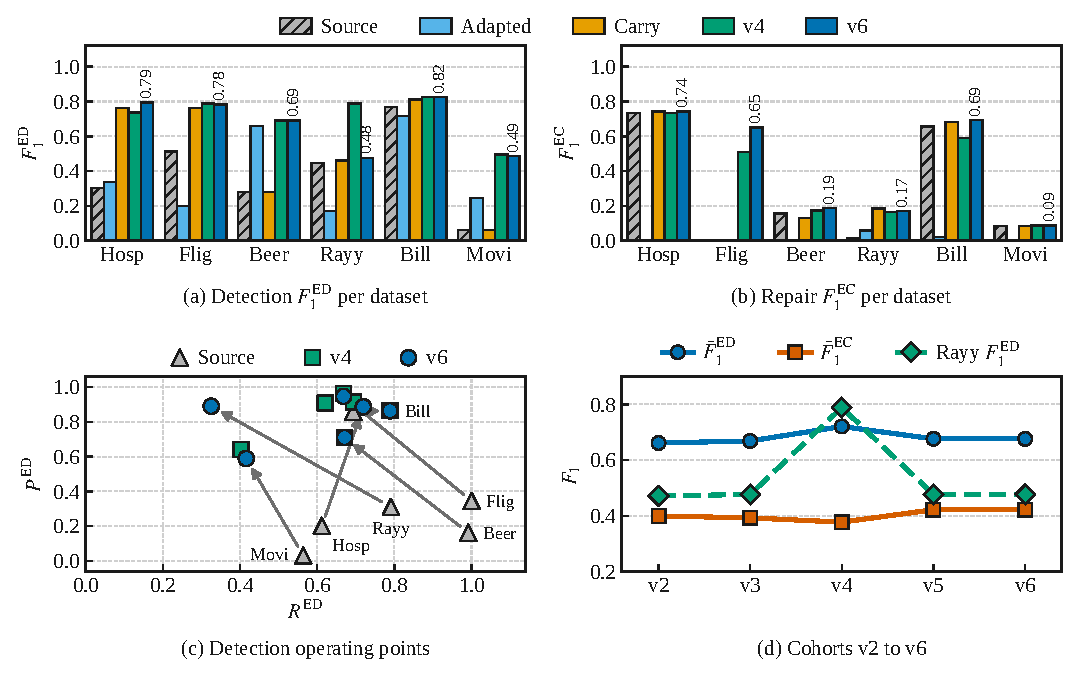
\includegraphics{figures/fig_benchmark.pdf}
\caption{Parallel and progressive benchmark results: (a) detection score $F_1^{\mathrm{ED}}$ per dataset; (b) repair score $F_1^{\mathrm{EC}}$ per dataset; (c) detection operating points, with one labeled arrow per dataset from source ZeroED (grey triangle) to v6 (blue circle) and green squares for v4; (d) macro scores $\bar{F}_1^{\mathrm{ED}}$ and $\bar{F}_1^{\mathrm{EC}}$ and the Rayyan detection score over the cohorts v2 to v6. In (a) and (b), hatched grey bars are source ZeroED and the sequential reconstruction, sky-blue bars are the adapted baselines, orange bars are the empty carry in (a) and the seeded carry in (b), green bars are v4, and blue bars are v6; the number above a blue bar is the score of v6.}
\label{fig:benchmark}
\end{figure*}

\subsection{Parallel Six-Dataset Comparison}
\label{subsec:exp_parallel}

Table~\ref{tab:main_benchmark} and Fig.~\ref{fig:benchmark}(a)--(c) compare the systems side by side.

\subsubsection{Error Detection}
Source ZeroED flags 157,253 of the 247,084 cells, and 139,328 of these flags are false positives. Its precision is 0.2017 on Hospital, 0.3451 on Flights, 0.1623 on Beers, 0.3107 on Rayyan, and 0.0318 on Movies, and its macro score is \SourceMacroED{}. The adapted detector reaches 0.3878 and does not improve on it. ZeroClean-Loop v6 flags 17,201 cells with 3,636 false positives and reaches \VsixMacroED{}, a gain of \VsixEDGain{} that is positive on every dataset: 49.07~pp on Hospital, 27.01~pp on Flights, 41.10~pp on Beers, 3.04~pp on Rayyan, 5.75~pp on Billionaire, and 42.76~pp on Movies.

Fig.~\ref{fig:benchmark}(c) shows the mechanism. Each arrow leads from the operating point of source ZeroED (grey triangle) to that of v6 (blue circle); green squares mark v4. All six arrows point upward, so precision rises on every dataset. Four arrows point to the left: recall falls from 1.0000 to 0.6683 on Flights, from 0.9918 to 0.6710 on Beers, from 0.7910 to 0.3254 on Rayyan, and from 0.5638 to 0.4162 on Movies. The gate thus trades recall for precision, and the trade is unfavorable on Rayyan, where v6 keeps only 3.04~pp of gain.

Version v4 reaches the higher macro score of \VfourMacroED{} because of Rayyan alone (0.7888 against 0.4765). On Hospital, v6 is 5.69~pp ahead: the format outlier promoter $G$ adds 105 flags, of which 81 are true errors. On Flights and Movies, v6 is 0.52~pp and 0.73~pp behind: the same promoter adds 55 flags on Flights, all on clean cells, and 493 flags on Movies, of which 83 are true errors. Beers and Billionaire are identical in both versions. Relative to the uncontrolled published reference, v6 is higher on Flights (0.7832 against 0.722) and Billionaire (0.8245 against 0.767) and lower on Hospital, Beers, Rayyan, and Movies; the published macro mean of 0.762 remains above both of our versions.

\subsubsection{Error Correction}
The sequential reconstruction reaches a macro repair score of \SeqMacroRepair{}. ZeroClean-Loop v6 reaches \VsixMacroRepair{}, which is \VsixRepairGain{} above the sequential reconstruction, 11.74~pp above the seeded carry, and 4.46~pp above v4. The gain over the sequential reconstruction is positive on all six datasets: 0.73~pp on Hospital, 64.91~pp on Flights, 3.17~pp on Beers, 15.45~pp on Rayyan, 3.47~pp on Billionaire, and 0.29~pp on Movies. The distribution is uneven. Flights contributes 64.91 of the 88.02 summed points; without Flights the mean gain is 4.62~pp, and the gains on Hospital and Movies are marginal. On Flights, the source consensus commits 2,989 edits of which 2,573 equal the reference ($P^{\mathrm{EC}} = 0.8608$, $R^{\mathrm{EC}} = 0.5230$), whereas the sequential reconstruction makes 4 correct edits. The seeded carry keeps the best repair score on Hospital (0.7432) and Rayyan (0.1862). Over the cohort, v6 has a macro repair precision of 0.7308 and a macro repair recall of 0.3308: it repairs about one third of the errors.

\subsection{Progressive Evolution Across Cohorts}
\label{subsec:exp_progressive}

% Auto-generated by scripts/generate_icde_tables.py from frozen evaluator-owned JSON artifacts.
% Do not edit by hand.
\begin{table}[t]
\centering
\caption{Progressive Evolution Across Frozen Study Cohorts. Flig and Rayy Give the Detection Score $F_1^{\mathrm{ED}}$ on Flights and Rayyan; Pos.\ EC Counts the Datasets on Which the Repair Score $F_1^{\mathrm{EC}}$ Exceeds the Sequential Reconstruction.}
\label{tab:trajectory}
\footnotesize
\setlength{\tabcolsep}{5pt}
\begin{tabular}{lrrrrr}
\toprule
\textbf{Study Cohort} & $\bar{F}_1^{\mathrm{ED}}$ & $\bar{F}_1^{\mathrm{EC}}$ & Flig & Rayy & Pos.\ EC \\
\midrule
Source and Sequential & 0.3948 & 0.2749 & 0.5131 & 0.4461 & -- \\
Source Loop v1 & 0.5729 & 0.2707 & 0.5374 & 0.2711 & 2/6 \\
Format Overlay v1 & 0.5977 & 0.2607 & 0.5370 & 0.2711 & 2/6 \\
Empty Carry & 0.5234 & 0.2668 & 0.7614 & 0.4607 & 2/6 \\
Seeded Carry & 0.5031 & 0.3042 & 0.6717 & 0.4606 & 4/6 \\
ZeroClean-Loop v2 & 0.6613 & 0.3992 & 0.7657 & 0.4711 & 5/6 \\
ZeroClean-Loop v3 & 0.6686 & 0.3924 & \textbf{0.7884} & 0.4765 & 5/6 \\
ZeroClean-Loop v4 & \textbf{0.7206} & 0.3770 & \textbf{0.7884} & \textbf{0.7888} & 4/6 \\
ZeroClean-Loop v5 & 0.6760 & \textbf{0.4216} & 0.7832 & 0.4765 & 6/6 \\
ZeroClean-Loop v6 & 0.6760 & \textbf{0.4216} & 0.7832 & 0.4765 & 6/6 \\
\bottomrule
\end{tabular}
\end{table}


Table~\ref{tab:trajectory} and Fig.~\ref{fig:benchmark}(d) follow the system through its frozen cohorts. In Fig.~\ref{fig:benchmark}(d), blue circles track $\bar{F}_1^{\mathrm{ED}}$, vermilion squares track $\bar{F}_1^{\mathrm{EC}}$, and green diamonds on the dashed line track the Rayyan detection score.

\emph{External Verifier Loops.} Source Loop v1 adds rounds of external LLM review to source ZeroED, and Format Overlay v1 adds reviewed format contracts to such a loop. They raise $\bar{F}_1^{\mathrm{ED}}$ from 0.3948 to 0.5729 and 0.5977, and $\bar{F}_1^{\mathrm{EC}}$ stays at 0.2707 and 0.2607, below the sequential reconstruction, with a repair score of 0.0004 on Flights.

\emph{Carry Arms.} The empty carry detects better than the seeded carry ($\bar{F}_1^{\mathrm{ED}}$ of 0.5234 against 0.5031; 0.7614 against 0.6717 on Flights), and the seeded carry repairs better ($\bar{F}_1^{\mathrm{EC}}$ of 0.3042 against 0.2668). Version v2 takes the detection scores of the empty arm, the sequential seed repairs, and the cached CTS candidates and adds the key-grouped source consensus: $\bar{F}_1^{\mathrm{ED}}$ rises to 0.6613, $\bar{F}_1^{\mathrm{EC}}$ to 0.3992, and the Flights repair score rises from 0.0004 to 0.5608.

\emph{Rule Union and Structural Promotion.} Version v3 evaluates the union of the cached and the fresh rule artifacts and raises the Flights detection score from 0.7657 to 0.7884. Version v4 adds the bibliographic promoter and raises the Rayyan detection score from 0.4765 to 0.7888 and $\bar{F}_1^{\mathrm{ED}}$ to 0.7206. Its repair score on Billionaire falls from 0.6838 to 0.5917: v4 admits 68 instead of 70 rules there, 633 candidate reviews end with a rule exception on the counterfactual tuple, a rejection that occurs in neither v3 nor v6, and the number of flagged cells without an edit rises from 1,855 to 2,442.

\emph{Generic Promotion and Weighted Repair.} Versions v5 and v6 replace the bibliographic promoter by the promoters of Section~\ref{subsec:det_structural} and the strict repair policy by the bound $\tau_{\mathrm{loss}}$ and the weighted guard. They report identical scores; v6 is the independently recounted cohort. $\bar{F}_1^{\mathrm{EC}}$ rises to 0.4216, and v5 and v6 are the only cohorts with a repair gain on all six datasets. $\bar{F}_1^{\mathrm{ED}}$ falls to 0.6760 because Rayyan returns to 0.4765. No cohort is best on both tasks: v4 has the highest macro detection score and v6 the highest macro repair score.

\subsection{Ablation Studies}
\label{subsec:exp_ablations}

% Auto-generated by scripts/generate_icde_tables.py from frozen evaluator-owned JSON artifacts.
% Do not edit by hand.
\begin{table}[t]
\centering
\caption{Component Ablation of the First Verification Pass on Frozen Inputs: Without Multi-Column Rules and FDs (w/o MC), Without Counterfactual Features (w/o CF), and With Both (Full).}
\label{tab:ablation}
\footnotesize
\setlength{\tabcolsep}{4.6pt}
\begin{tabular}{lrrrrrr}
\toprule
& \multicolumn{2}{c}{\textbf{w/o MC}} & \multicolumn{2}{c}{\textbf{w/o CF}} & \multicolumn{2}{c}{\textbf{Full}} \\
\cmidrule(lr){2-3} \cmidrule(lr){4-5} \cmidrule(lr){6-7}
\textbf{Dataset} & $F_1^{\mathrm{ED}}$ & $F_1^{\mathrm{EC}}$ & $F_1^{\mathrm{ED}}$ & $F_1^{\mathrm{EC}}$ & $F_1^{\mathrm{ED}}$ & $F_1^{\mathrm{EC}}$ \\
\midrule
Hospital & \textbf{0.7660} & 0.7395 & \textbf{0.7660} & 0.7405 & \textbf{0.7660} & \textbf{0.7414} \\
Flights & 0.0008 & 0.0004 & 0.0045 & \textbf{0.0036} & \textbf{0.5374} & 0.0004 \\
Beers & \textbf{0.6928} & 0.1275 & 0.6924 & 0.1168 & 0.6924 & \textbf{0.1286} \\
Rayyan & \textbf{0.2711} & 0.1855 & \textbf{0.2711} & 0.1860 & \textbf{0.2711} & \textbf{0.1875} \\
Billionaire & 0.8223 & 0.4088 & 0.8292 & \textbf{0.5226} & \textbf{0.8357} & 0.5089 \\
Movies & 0.2972 & 0.0226 & 0.3098 & \textbf{0.0258} & \textbf{0.3319} & 0.0190 \\
\midrule
\textbf{Macro Mean} & 0.4750 & 0.2474 & 0.4788 & \textbf{0.2659} & \textbf{0.5724} & 0.2643 \\
\bottomrule
\end{tabular}
\end{table}


\begin{figure*}[t]
\centering
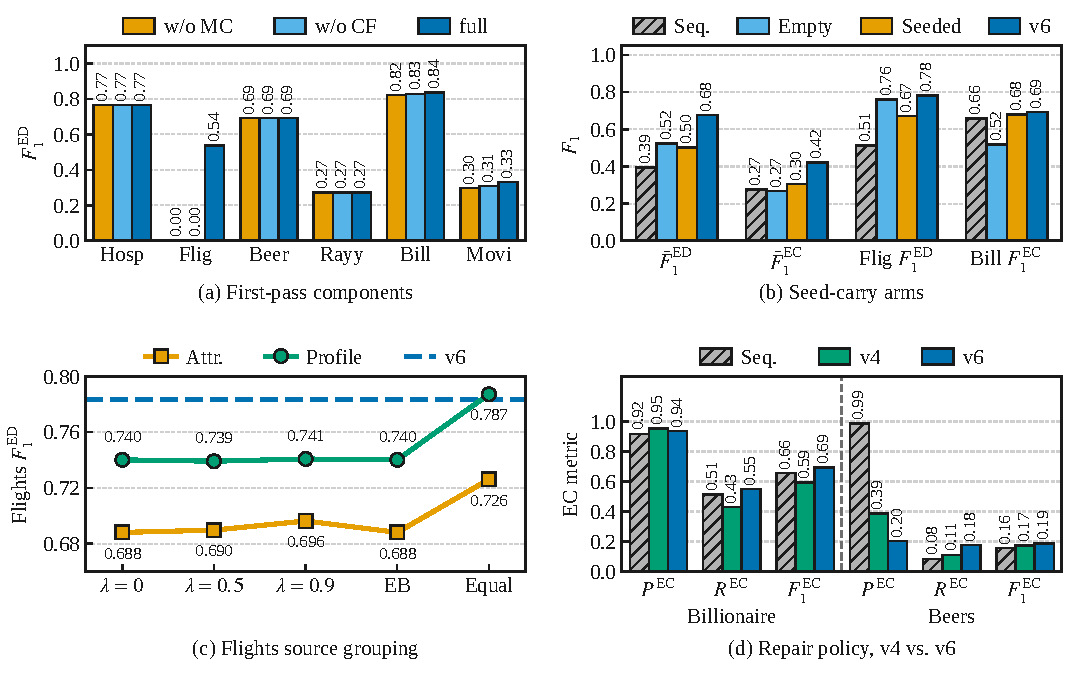
\includegraphics{figures/fig_ablation.pdf}
\caption{Ablation studies: (a) detection score of the first verification pass without multi-column rules and FDs (w/o MC), without counterfactual features (w/o CF), and with both (full); (b) seed-carry arms against the sequential reconstruction (Seq.) and v6 on two macro scores, the Flights detection score, and the Billionaire repair score; (c) Flights detection score of the source reliability model under attribute-near (Attr.) and profile-complete (Profile) source grouping for three pooling strengths $\lambda$, empirical Bayes selection (EB), and equal reliability (Equal), with v6 as the dashed reference; (d) repair precision $P^{\mathrm{EC}}$, recall $R^{\mathrm{EC}}$, and score $F_1^{\mathrm{EC}}$ of the sequential reconstruction, v4, and v6 on Billionaire and Beers. Numbers above bars and next to markers are the plotted scores.}
\label{fig:ablation}
\end{figure*}

\subsubsection{Components of the First Verification Pass}
Table~\ref{tab:ablation} and Fig.~\ref{fig:ablation}(a) report a matched ablation of the earlier verified loop on frozen inputs. It repeats the first verification pass without multi-column rules and FDs (orange bars) and without counterfactual features (sky-blue bars); it does not ablate v6 itself. Removing multi-column evidence lowers $\bar{F}_1^{\mathrm{ED}}$ by 9.74~pp, from 0.5724 to 0.4750, and removing counterfactual features lowers it by 9.36~pp, to 0.4788. Nearly the whole difference arises on Flights, where the detection score falls from 0.5374 to 0.0008 and 0.0045. On the other five datasets the variants differ by at most 3.47~pp, and Hospital and Rayyan do not change. In repair, removing multi-column evidence costs 1.69~pp of $\bar{F}_1^{\mathrm{EC}}$ and 10.01~pp on Billionaire (0.5089 to 0.4088). Removing counterfactual features does not lower the repair score: $\bar{F}_1^{\mathrm{EC}}$ is 0.2659 against 0.2643. In this pass, counterfactual features pay off in detection on the multi-source table and show no repair benefit.

\begin{figure*}[t]
\centering
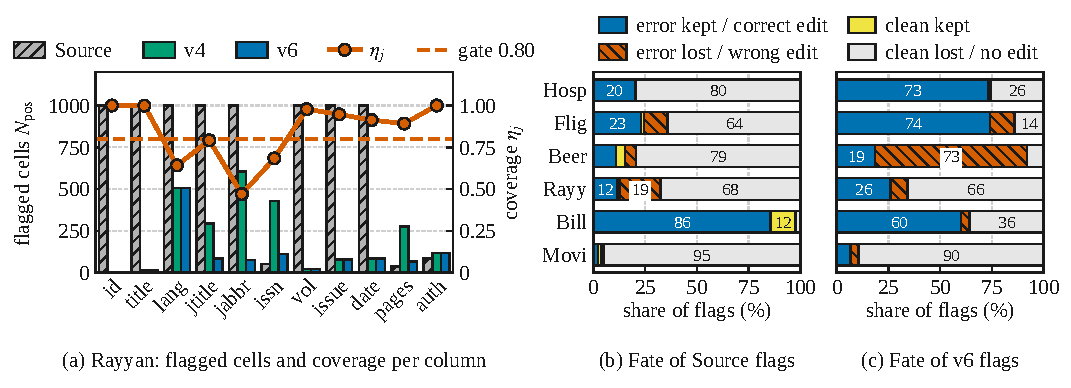
\includegraphics{figures/fig_diagnostics.pdf}
\caption{Cell-level diagnostics: (a) flagged cells $N_{\mathrm{pos}}$ per Rayyan column for source ZeroED (hatched grey), v4 (green), and v6 (blue), with the column coverage $\eta_j$ (vermilion line, right axis) and the gate of 0.80 (dashed); (b) fate of the flags of source ZeroED under v6; (c) fate of the flags of v6 in repair. In (b), blue is an erroneous cell that stays flagged, yellow a clean cell that stays flagged, hatched vermilion an erroneous cell that loses its flag, and grey a clean cell that loses its flag; in (c), blue is a correct edit, hatched vermilion a wrong edit, and grey a flagged cell without an edit; numbers inside the bars are shares in percent.}
\label{fig:diagnostics}
\end{figure*}

\subsubsection{Seed-Carry Arms}
Fig.~\ref{fig:ablation}(b) places the empty carry (sky blue) and the seeded carry (orange) between the sequential reconstruction (hatched grey) and v6 (blue). Neither arm reaches v6 on a macro score. The seeded carry is close to v6 on the Billionaire repair score (0.6812 against 0.6924), and the empty carry is close on the Flights detection score (0.7614 against 0.7832); v6 obtains both properties in one system.

\subsubsection{Source Grouping on Flights}
Fig.~\ref{fig:ablation}(c) reports a preregistered, detection-only study of the source reliability model. Attribute-near grouping (orange squares) merges sources per attribute when they agree on at least $98~\%$ of at least 12 shared flights; profile-complete grouping (green circles) merges sources only when their complete reports coincide. The settings are three pooling strengths $\lambda \in \{0, 0.5, 0.9\}$ of a hierarchical prior, a nested Empirical Bayes (EB) selection of $\lambda$, and an equal reliability control. Profile-complete grouping exceeds attribute-near grouping by 4.45~pp to 6.12~pp at every setting. Learned reliability does not help: the equal control is the best setting under both groupings (0.7261 and 0.7873) and exceeds the learned settings by 2.99~pp to 4.81~pp. In line with this result, v6 accepts a consensus value only when unweighted source counts and weighted votes name the same winner; its detection score of 0.7832 is 0.40~pp below the best control.

\subsubsection{Repair Policy}
Fig.~\ref{fig:ablation}(d) compares the strict policy of v4 (green) with the policy of v6 (blue) and the sequential reconstruction (hatched grey). On Billionaire, with 70 admitted rules, v6 commits 3,088 edits of which 2,892 are correct, against 2,366 edits and 2,258 correct edits in v4. Recall rises from 0.4288 to 0.5492, precision falls from 0.9544 to 0.9365, and the repair score rises by 10.06~pp to 0.6924. The gain originates at the candidate level: beyond the 633 rule exceptions, v4 rejects candidates for a new rule violation (73 reviews), a negative score (32), and a loss of FD support (27), and none of these rejections remains in v6. The weighted row guard is a secondary factor. Over the six datasets it rolls back 8 of 6,034 edited rows (v4: 1 of 4,292), and it commits 38 rows that introduce a rule violation, 37 of them on Billionaire; these rows carry 88 edits of which 67 are correct. On Beers, v6 removes the catalog gate of v4 and adds 180 correct and 1,458 wrong edits: recall rises from 0.1112 to 0.1751, precision falls from 0.3874 to 0.2016, and the repair score rises by 1.46~pp. The sequential reconstruction has the highest precision on Beers (0.9876) at a recall of 0.0845.

\subsection{Diagnostic Analysis and Limitations}
\label{subsec:exp_diagnostics}

This section accounts for every flag of the source detector and of v6 and states where the method fails.

\subsubsection{What the Gate Removes and What It Costs}
Fig.~\ref{fig:diagnostics}(b) partitions the 157,253 flags of source ZeroED by their fate under v6. The detector drops 141,212 flags, of which 135,955 lie on clean cells ($96.3~\%$) and 5,257 on erroneous cells. The dropped errors are the cost of the gate: 1,632 on Flights, 1,593 on Rayyan, 1,100 on Movies, and 926 on Beers. They are cells without any dirty-only witness, such as the fourth cell of Fig.~\ref{fig:trace}(a): a well-formed wrong time for which no actionable consensus value exists. On Billionaire no column is gated and 107 flags are dropped.

\subsubsection{Rayyan: Missing Values Below the Coverage Gate}
Fig.~\ref{fig:diagnostics}(a) shows the flagged cells per Rayyan column. Source ZeroED flags all 1,000 tuples in eight of the eleven columns (8,176 flags, $P^{\mathrm{ED}} = 0.3107$). Version v6 keeps 1,175 flags with $P^{\mathrm{ED}} = 0.8894$ and $R^{\mathrm{ED}} = 0.3254$, which leaves 2,166 false negatives. Version v4 keeps 2,438 flags, of which 2,228 are true errors. The 1,263 flags that only v4 raises lie in four columns: 529 in the journal abbreviation, 317 in the International Standard Serial Number (ISSN), 209 in the pagination, and 208 in the journal title. Of these cells, 1,160 are empty and 1,183 are true errors. Version v4 flags them through column-name tokens for bibliographic metadata. Version v6 promotes an empty cell only in a fallback column with $\eta_j \ge 0.80$: the journal abbreviation ($\eta_j = 0.471$) and the journal title ($\eta_j = 0.792$) lie below the gate, and the ISSN and the pagination are not fallback columns ($\gamma_j$ of 0.052 and 0.038). The three fallback columns above the gate hold 162 empty cells that other witnesses already retain, so the fallback promoter adds no flag on Rayyan. On Movies the same promoter is correct: all 1,009 flags that it corroborates are true errors. A single coverage threshold therefore does not separate corrupted missing values from legitimately optional ones, and the rule that separates them on Rayyan depends on column names. Version v6 still consults column-name tokens in its open-vocabulary test, so a treatment of missing values that is free of schema names remains open. A further 722 false negatives of both versions are non-empty values of the creation date column that carry no witness.

\subsubsection{Repair: Abstention and Wrong Edits}
Fig.~\ref{fig:diagnostics}(c) partitions the 17,201 flags of v6: 7,046 receive a correct edit ($41.0~\%$), 2,834 a wrong edit ($16.5~\%$), and 7,321 no edit ($42.6~\%$). On Movies, 3,953 of the 4,413 flags stay unedited. The candidate pool draws only on observed dirty values and seed proposals, and only 808 Movies cells receive a candidate at all; the errors concentrate in free-text attributes (1,682 in the description, 1,047 in the filming locations, and 824 in the creator). Of the 294 correct edits, 287 lie in the year, genre, and duration attributes. On Beers, 1,953 of the 2,446 edits are wrong ($79.8~\%$), and 1,947 of them lie in two attributes. In the volume attribute, 1,486 edits install the most frequent dirty form \texttt{12.0 oz.}, whereas the reference form is \texttt{12.0 oz}; 621 of these edits overwrite a cell that is already clean. In the ABV attribute, 440 edits strip the percent sign (\texttt{0.05\%} becomes \texttt{0.05}), whereas the reference holds a value of another precision (\texttt{0.045}). Under exact-string evaluation, the dominant dirty format is not the reference format, and the dirty table alone does not reveal this.

\subsubsection{Measured Effect of the Feedback Channels}
The counterfactual promotion and demotion rules of Section~\ref{subsec:rep_counterfactual} change 0 cells on each of the six datasets, although candidates are evaluated for 15,255 triggered cells. The reported scores of v6 therefore owe nothing to these two rules. The feedback that the benchmark measures is the consensus contradiction witness: it fires on 2,436 Flights cells, retains 2,407 inherited flags, and promotes 29 unflagged cells. It fires on no cell of the other five datasets, on which key discovery finds no entity key with a source column. On the benchmark, closing the loop thus benefits the multi-source table, and the single-source tables profit from the gate, the promoters, and the repair policy.

\subsubsection{Running Time}
Table~\ref{tab:datasets} reports the inference time $t_{\mathrm{inf}}$ of v6 on one thread. The six tables take 194.87~s in total, from 8.68~s on Rayyan to 82.46~s on Movies, the table with the most tuples. These times cover Algorithm~\ref{alg:loop} on the pinned inputs and exclude the LLM calls for rule synthesis and the upstream runs that produce the inherited scores, the seed repairs, and the CTS pools.

\subsubsection{Threats to Validity}
Each cohort is a single run with one LLM and one seed, so no variance estimate is available. The sequential baseline is a reconstruction, and the published reference is uncontrolled. ZeroClean-Loop v6 consumes the scores and candidates of earlier pipeline stages as pinned inputs and is not evaluated as a standalone system. The component and grouping ablations measure earlier loop variants and not v6.

\section{Related Work}
\label{sec:related}

\subsection{Rule-Based, Holistic, and Probabilistic Data Repair}
\label{subsec:rel_holistic}

Constraint-based cleaning systems detect and repair violations of FDs, CFDs~\cite{fan2008conditional}, denial constraints~\cite{chu2013holistic}, and fixing rules~\cite{wang2014towards}. Bohannon et al.~\cite{bohannon2005cost} introduce cost-based value modification, and NADEEF~\cite{dallachiesa2013nadeef} and LLUNATIC~\cite{geerts2013llunatic} generalize holistic repair over heterogeneous constraints. Guided Data Repair~\cite{yakout2011guided} and ActiveClean~\cite{krishnan2016activeclean} incorporate human feedback, and HoloClean~\cite{rekatsinas2017holoclean} unifies integrity constraints, master data, and statistics in a probabilistic model. These systems need experts who author rules or supply master data before ingestion. ZeroClean-Loop synthesizes executable constraints and discovers FDs from the dirty table and, like HoloClean, treats a repair as a decision under several signals; it differs in that it verifies each candidate by execution on a counterfactual tuple.

\subsection{Supervised and Multi-Source Cleaning}
\label{subsec:rel_supervised}

Raha~\cite{mahdavi2019raha} trains per-column detectors from 20 labeled tuples, and Baran~\cite{mahdavi2020baran} learns value, vicinity, and domain correction models from the same budget; our vicinity and domain features follow this decomposition without labels. HoloDetect~\cite{heidari2019holodetect} uses data augmentation for few-shot detection, and confident learning~\cite{northcutt2021confident} estimates label noise. Truth discovery~\cite{dong2009data,li2014confidence} estimates source reliability jointly with entity truths. ZeroClean-Loop grounds source quality in dirty-only format validity, chronological order, and leave-one-source-out agreement (Eq.~\eqref{eq:source_consensus}), and our grouping study shows that equal reliability is a strong control on Flights.

\subsection{Foundation Models for Tabular Cleaning}
\label{subsec:rel_llm}

Narayan et al.~\cite{narayan2022can} show that foundation models perform data wrangling tasks from prompts. ZeroED~\cite{ni2025zeroed} and ZeroEC~\cite{chen2025zeroec} use an LLM to generate verification functions and contextual repairs without labels. Section~\ref{sec:experiments} shows that the open-loop cascade of the two systems inherits the empty-predicate degeneracy and commits unverified substitutions. ZeroClean-Loop keeps the scores of ZeroED and the CTS candidates and seed repairs of ZeroEC as inputs and adds the gate, the counterfactual verification, and the row guard between them.

\section{Conclusion}
\label{sec:conclusion}

This paper presents ZeroClean-Loop, a closed-loop error detection and repair system for autonomous tabular data ingestion. It gates inherited classifier scores with dirty-only witnesses, verifies every candidate repair on a counterfactual copy of its tuple, returns repair-side consensus evidence to the detector, and commits rows under a weighted guard. On six benchmark datasets, ZeroClean-Loop v6 reaches a macro detection score of \VsixMacroED{}, which is \VsixEDGain{} above source ZeroED, and a macro repair score of \VsixMacroRepair{}, which is \VsixRepairGain{} above the sequential reconstruction, with a repair gain on every dataset. The analysis also fixes the limits of these results: the gate drops 5,257 true errors together with 135,955 false flags, the removal of column-name rules costs 31.23~pp of detection score on Rayyan, the dominant dirty format misleads repair on Beers, and the counterfactual feedback rules have no measured effect, so the measured benefit of the closed loop is confined to the multi-source table. Missing values in moderately sparse columns and feedback for single-source tables are the open problems that follow directly from these measurements.

\section*{Acknowledgment of AI-Generated Content}
The author used Generative Artificial Intelligence (AI) tools, Cursor and Claude, to run the experiments reported in this paper. The author wrote the text and produced the figures of this manuscript.

\IEEEtriggeratref{11}
\bibliographystyle{IEEEtran}
\bibliography{references}
\end{document}
